\section{Vista de Desarrollo}
En la siguiente figura \ref{fig:Diagrama de Componentes - Vista de Desarrollo} se muestra el diagrama de componentes del sistema, donde se muestran los diversos componentes e interfaces. Partimos de una principal, el IniciarSesion; por la cual se va a interactuar a la visualización del menú por medio de la pantallaMenu. Además este componente tiene una conexión a la base de datos para verificar la identidad del usuario y darle acceso o no al sistema. 
\\
Por medio del componente de VisualizarMenu, a través de la interfaz pantallaMenu, el usuario puede elegir una opción que el sistema ofrece. El componente de VisualizarAgenda tiene relación con los siguientes componentes e interfaces: 
\begin{itemize}
	\item \textbf{RegistrarVehiculo:} Por medio de la interfaz pantallaRegVehiculo, se tiene una conexión con este componente para el posterior registro en la base de datos.
	\item \textbf{ActualizarVehiculo:} Por medio de la interfaz pantallaActVehiculo, se tiene la conexión con este componente para poder modificar un registro de la base de datos.
	\item \textbf{EliminarVehiculo:} Por medio de la interfaz pantallaElimVehiculo, se tiene conexión con este componente para poder eliminar un registro de un vehículo.
	\item \textbf{BuscarVehiculo:} A través de la interfaz pantallaBusVehiculo, se tiene conexión con este componente para poder buscar un registro de un vehículo en especifico. 
\end{itemize}
Por otro lado, se tiene el componente VisualizarRefacciones, con el cual se obtiene una conexión por medio de la interfaz pantallaGestRef. Que a su vez, se conecta al componente RegistrarSolicitud por medio de la interfaz pantallaRegSol. Esto con la finalidad de visualizar si existen refacciones en almacén del taller o solicitar alguna. 
\begin{figure}[!h]
	\centering
	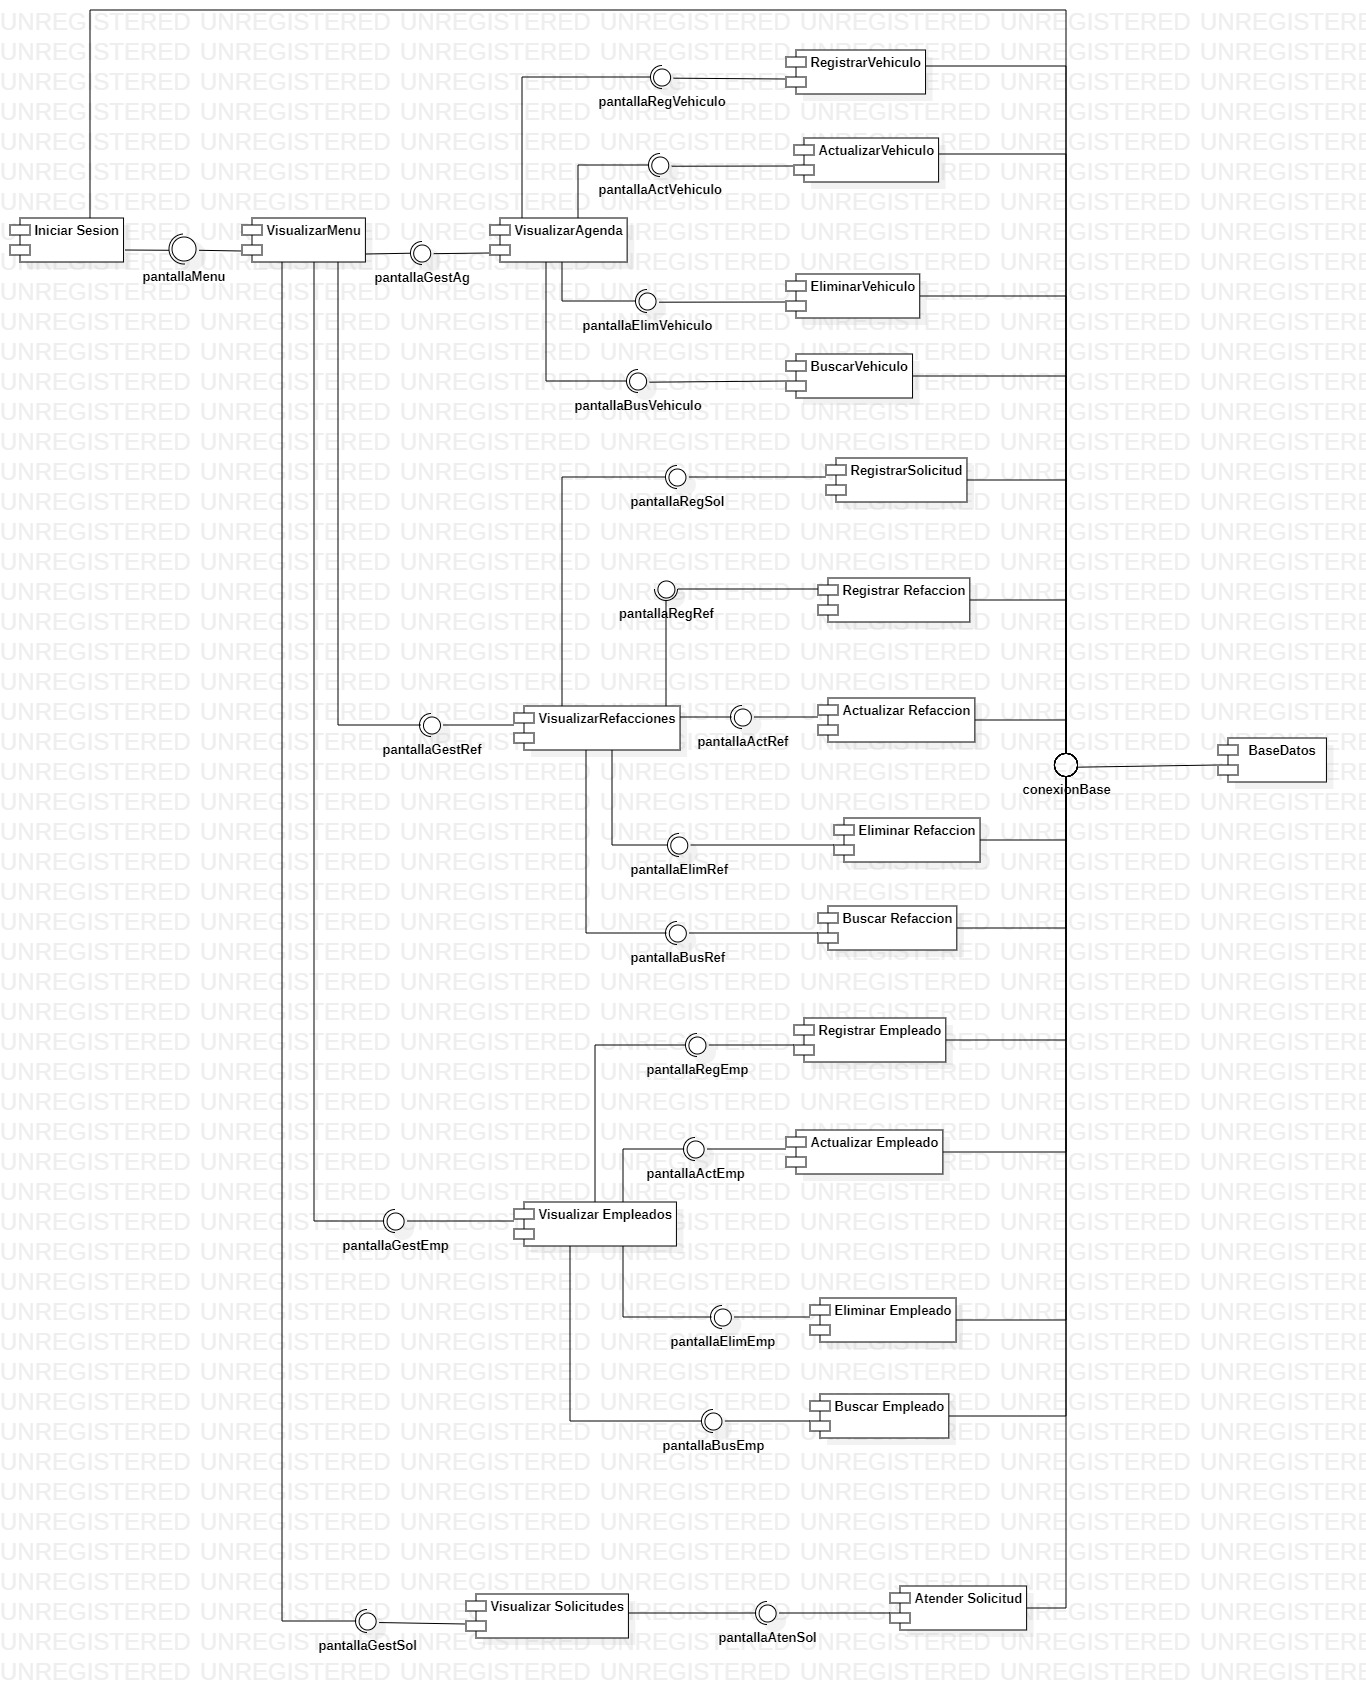
\includegraphics[width=1.3\textwidth]{./diseno/vdesarrollo/imagenes/vistaDesarrollo}
	\caption{Diagrama de Componentes - Vista de Desarrollo}
	\label{fig:Diagrama de Componentes - Vista de Desarrollo}
\end{figure}
\clearpage